\documentclass[a4paper]{article}
\usepackage[a4paper,margin=0mm]{geometry}
\usepackage{fontspec}
\usepackage{unicode-math}
\usepackage{tikz}
\usepackage[table]{xcolor}
\usepackage[absolute]{textpos}
\usepackage{array}
\usepackage{multirow}

\setmainfont{Libertinus Serif}
\setsansfont{Libertinus Sans}
\setmathfont{Libertinus Math}

\definecolor{accent}{HTML}{0F6A52}
\definecolor{badge}{HTML}{A9CFC2}
\definecolor{ink}{HTML}{2A2E30}

\setlength{\TPHorizModule}{1mm}
\setlength{\TPVertModule}{1mm}
\setlength{\parindent}{0pt}
\setlength{\parskip}{0pt}
\emergencystretch=3em
\abovedisplayskip=4pt plus 2pt minus 2pt \belowdisplayskip=4pt plus 2pt minus 2pt \abovedisplayshortskip=2pt \belowdisplayshortskip=2pt
\pagestyle{empty}

\newcommand{\LCOL}{16mm}
\newcommand{\RCOL}{111mm}
\newcommand{\COLW}{83mm}

\newcommand{\topicheader}[2]{%
\begin{textblock*}{194mm}(16mm,10mm)
\begin{tikzpicture}
\node[fill=accent,text=white,font=\sffamily\bfseries\fontsize{13}{13}\selectfont,
      minimum width=9mm,minimum height=9mm,inner sep=0pt] at (4.5mm,-4.5mm) {#1};
\node[font=\sffamily\bfseries\fontsize{15}{16}\selectfont,text=ink,anchor=west] at (12mm,-4.5mm) {#2};
\end{tikzpicture}
\end{textblock*}
\begin{textblock*}{194mm}(16mm,22.5mm)

\begin{tikzpicture}
\fill[accent] (0,0) rectangle (194mm,0.5mm);
\end{tikzpicture}
\end{textblock*}
}

\newcommand{\pagefooter}[1]{%
\begin{textblock*}{194mm}(8mm,286.41mm)
  
\begin{tikzpicture}
    \fill[accent] (0,0) rectangle (194mm,0.6mm);
  \end{tikzpicture}
\end{textblock*}
\begin{textblock*}{63.59mm}(8mm,288.27mm)
  {\sffamily\bfseries\color{accent}\fontsize{13}{16}\selectfont SAT 1200+}
\end{textblock*}
\begin{textblock*}{10mm}(188mm,288.27mm)
  \centering{\sffamily\color{accent}\fontsize{14}{16}\selectfont #1}
\end{textblock*}
}

\newcommand{\colrule}[2]{%
\begin{textblock*}{1mm}(105mm,#1mm)
\begin{tikzpicture}
\draw[black!65,line width=0.5pt] (0,0) -- (0,#2mm);
\end{tikzpicture}
\end{textblock*}
}

\newcommand{\setkicker}[2]{%
{\sffamily\bfseries\fontsize{12}{14}\selectfont #1.}\ {\itshape\fontsize{11}{14}\selectfont\color{black!75} #2}\par\vspace{2mm}%
}

\setlength{\fboxsep}{1.4pt}
\setlength{\fboxrule}{0.5pt}
\newcommand{\pnum}[1]{\fcolorbox{ink}{white}{\sffamily\bfseries\fontsize{8}{8}\selectfont #1}~}

% ---- SAT-style multiple-choice block (2x2 grid of short choices) ----
\newcommand{\satq}[6]{%
\noindent\pnum{#1} #2\par\nobreak\vspace{2mm}%
\noindent\hspace*{7mm}\begin{tabular}[t]{@{}p{32mm}p{32mm}@{}}
(A) #3 & (B) #4 \\[2mm]
(C) #5 & (D) #6 \\
\end{tabular}\par\vspace{5.5mm}%
}

% ---- stacked choices for long ones ----
\newcommand{\satqw}[6]{%
\noindent\pnum{#1} #2\par\nobreak\vspace{2mm}%
\noindent\hspace*{7mm}(A) #3\par\vspace{1.6mm}%
\noindent\hspace*{7mm}(B) #4\par\vspace{1.6mm}%
\noindent\hspace*{7mm}(C) #5\par\vspace{1.6mm}%
\noindent\hspace*{7mm}(D) #6\par\vspace{5.5mm}%
}

% ---- student-produced response (grid-in) ----
\newcommand{\satg}[2]{%
\noindent\pnum{#1} {\sffamily\bfseries\fontsize{7}{8}\selectfont\color{accent}GRID-IN}\ #2\par\nobreak\vspace{2.5mm}%
\noindent\hspace*{7mm}{\sffamily\fontsize{8.5}{10}\selectfont Answer:}\ \rule[-1.2mm]{28mm}{0.4pt}\par\vspace{5.5mm}%
}

% ---- worked-solution entry ----
\newcommand{\solitem}[4]{%
\noindent\pnum{#1} {\bfseries #2}\ —\ #3\ {\itshape\color{accent}[#4]}\par\vspace{2.1mm}%
}

\usetikzlibrary{arrows.meta}
\newsavebox{\figsave}
\newcommand{\figbox}[1]{\par\vspace{1.8mm}\sbox{\figsave}{#1}\noindent\hfill\ifdim\wd\figsave>\hsize\resizebox{\hsize}{!}{\usebox{\figsave}}\else\usebox{\figsave}\fi\hfill\null\par\vspace{0.8mm}}
\arrayrulecolor{accent}
\setlength{\arrayrulewidth}{0.7pt}
\renewcommand{\arraystretch}{1.3}

\usepackage{multicol}
\usepackage{fancyhdr}
\usepackage{needspace}
\newcommand{\pgoff}{0}
\renewcommand{\solitem}[4]{\noindent\parbox[t]{\linewidth}{\raggedright\pnum{#1} {\bfseries #2}\ ---\ #3\ {\itshape\color{accent}[#4]}}\par\vspace{3.6mm}}
\newcommand{\solkicker}[2]{\Needspace{38mm}\vspace{1.5mm}{\sffamily\bfseries\fontsize{12.5}{15}\selectfont #1.}\ {\itshape\fontsize{11}{14}\selectfont\color{black!75} #2}\par\vspace{3mm}}
\renewcommand{\satqw}[6]{%
\noindent\pnum{#1} #2\par\nobreak\vspace{2mm}%
\noindent\hangindent=13mm\hangafter=1\hspace*{7mm}(A)~#3\par\vspace{1.6mm}%
\noindent\hangindent=13mm\hangafter=1\hspace*{7mm}(B)~#4\par\vspace{1.6mm}%
\noindent\hangindent=13mm\hangafter=1\hspace*{7mm}(C)~#5\par\vspace{1.6mm}%
\noindent\hangindent=13mm\hangafter=1\hspace*{7mm}(D)~#6\par\vspace{5.5mm}%
}
\newcommand{\solkitem}[5]{\noindent\parbox[t]{\linewidth}{\vspace{1.5mm}{\sffamily\bfseries\fontsize{12.5}{15}\selectfont #1.}\ {\itshape\fontsize{11}{14}\selectfont\color{black!75} Worked solutions}\par\vspace{3mm}\raggedright\pnum{#2} {\bfseries #3}\ ---\ #4\ {\itshape\color{accent}[#5]}}\par\vspace{3.6mm}}
\fancypagestyle{solstyle}{\fancyhf{}\renewcommand{\headrulewidth}{0pt}\renewcommand{\footrulewidth}{0pt}%
 \fancyhead[L]{\topicheader{8}{Hard Circles, Area \& Volume}}%
 \fancyfoot[L]{\pagefooter{\the\numexpr\value{page}+\pgoff\relax}}}

\newwrite\mw \immediate\openout\mw=meas.txt
\newcommand{\meas}[2]{\setbox0=\vbox{\hsize=83mm\fontsize{10}{12.5}\selectfont\noindent #2}\immediate\write\mw{#1 \the\dimexpr\ht0+\dp0\relax}}
\begin{document}
\meas{S1.1}{\satq{1}{The graph of $(x-2)^2+(y+5)^2=36$ in the $xy$-plane is a circle. What is the length of a diameter of the circle?}{$6$}{$12$}{$36$}{$72$}}
\meas{S1.2}{\satq{2}{A circle in the $xy$-plane has center $(1,-2)$ and radius $5$. Which of the following points lies \emph{inside} the circle?}{$(3,0)$}{$(-3,-5)$}{$(1,3)$}{$(6,1)$}}
\meas{S1.3}{\satg{3}{A circle has radius $9$. An arc of the circle has a central angle of $80^\circ$, and the length of the arc is $k\pi$. What is the value of $k$?}}
\meas{S1.4}{\satq{4}{A circle has a diameter of $24$. A sector of this circle has an area of $60\pi$. What is the measure, in degrees, of the central angle of the sector?}{$37.5$}{$60$}{$75$}{$150$}}
\meas{S1.5}{\satq{5}{Points $A$ and $B$ lie on a circle with center $O$, and $\angle AOB=100^\circ$. Point $C$ lies on the \emph{major} arc $AB$ (the longer arc). What is the measure, in degrees, of $\angle ACB$?}{$50^\circ$}{$100^\circ$}{$130^\circ$}{$200^\circ$}}
\meas{S1.6}{\satq{6}{A sphere has a volume of $288\pi$ cubic centimeters. What is the surface area, in square centimeters, of the sphere?}{$36 \pi$}{$72 \pi$}{$144 \pi$}{$576 \pi$}}
\meas{S1.7}{\satq{7}{A tank shaped like a rectangular box is $2$ m long, $1.5$ m wide and $0.8$ m deep. How many liters of water does it hold when full? ($1$ cubic meter $=1000$ liters)}{$2.4$}{$240$}{$2{,}400$}{$24{,}000$}}
\meas{S1.8}{\satq{8}{Two right circular cones are similar. The height of the larger cone is $3$ times the height of the smaller cone, and the smaller cone has a volume of $40$ cubic centimeters. What is the volume, in cubic centimeters, of the larger cone?}{$3{,}240$}{$1{,}080$}{$360$}{$120$}}
\meas{S1.9}{\satg{9}{An arc of length $2\pi$ lies on a circle of radius $6$. What is the measure, in degrees, of the central angle that intercepts the arc?}}
\meas{S1.10}{\satq{10}{A region is made of a $10$-by-$6$ rectangle together with a semicircle whose diameter is a $6$-unit side of the rectangle (the semicircle lies outside the rectangle). What is the area of the region?}{$60 + 36 \pi$}{$60 + 18 \pi$}{$60 + 9 \pi$}{$60 + \frac{9 \pi}{2}$}}
\meas{S1.11}{\satq{11}{Water is pumped into an empty cylindrical tank with a base radius of $4$ feet at a constant rate of $24\pi$ cubic feet per minute. By how many feet does the water level rise each minute?}{$0.375$}{$1.5$}{$3$}{$6$}}
\meas{S1.12}{\satg{12}{The equation $x^2+y^2-6x+10y+18=0$ defines a circle in the $xy$-plane. What is the radius of the circle?}}
\meas{S2.1}{\satq{1}{In the $xy$-plane, the graph of $x^2+y^2+8x-2y+k=0$ is a circle with radius $5$. What is the value of $k$?}{$-8$}{$8$}{$12$}{$42$}}
\meas{S2.2}{\satg{2}{The graph of $x^2+y^2-4x+6y-12=0$ is a circle in the $xy$-plane that crosses the $x$-axis at two points. What is the distance between these two points?}}
\meas{S2.3}{\satq{3}{In the $xy$-plane, a circle has center $(2,-1)$. A line is tangent to the circle at the point $(5,3)$. Which of the following points also lies on this line?}{$(9,6)$}{$(8,7)$}{$(9,0)$}{$(8,-1)$}}
\meas{S2.4}{\satq{4}{In the $xy$-plane, the circle $x^2+y^2=k$ is tangent to the line $3x-4y=40$. What is the value of $k$?}{$64$}{$8$}{$40$}{$1{,}600$}}
\meas{S2.5}{\satg{5}{A circle has radius $17$. Chord $AB$ has length $30$ and $M$ is the midpoint of $AB$. The line through the center $O$ and $M$ meets the circle again at point $N$ on the short arc $AB$ (see the figure). What is the length of $\overline{MN}$?\figbox{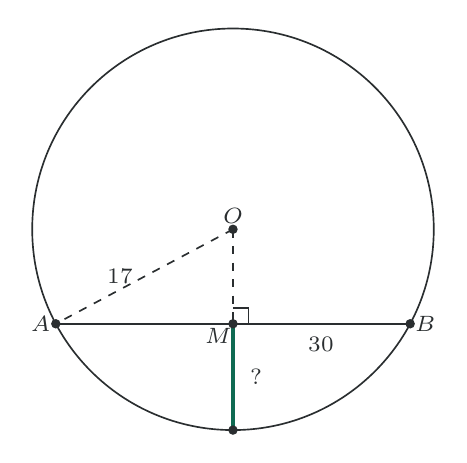
\begin{tikzpicture}[line width=0.6pt,ink,every node/.style={font=\footnotesize}]
\draw (0.000mm,0.000mm) circle (25.500mm);
\draw (-22.500mm,-12.000mm) -- (22.500mm,-12.000mm);
\draw[dashed] (0.000mm,0.000mm) -- (0.000mm,-12.000mm);
\draw[dashed] (0.000mm,0.000mm) -- (-22.500mm,-12.000mm);
\draw[accent,line width=1.4pt] (0.000mm,-12.000mm) -- (0.000mm,-25.500mm);
\draw[ink,line width=0.4pt] (0.000mm,-10.000mm) -- (2.000mm,-10.000mm) -- (2.000mm,-12.000mm);
\fill[ink] (0.000mm,0.000mm) circle (0.6mm); \node[above,inner sep=1.5pt] at (0.000mm,0.000mm) {$O$};
\fill[ink] (-22.500mm,-12.000mm) circle (0.6mm); \node[left,inner sep=1.5pt] at (-22.500mm,-12.000mm) {$A$};
\fill[ink] (22.500mm,-12.000mm) circle (0.6mm); \node[right,inner sep=1.5pt] at (22.500mm,-12.000mm) {$B$};
\fill[ink] (0.000mm,-12.000mm) circle (0.6mm); \node[below left,inner sep=1.5pt,xshift=0.5pt] at (0.000mm,-12.000mm) {$M$};
\fill[ink] (0.000mm,-25.500mm) circle (0.6mm);
\node[below=1pt] at (11.250mm,-12.000mm) {$30$};
\node[left=0.5pt] at (-11.250mm,-6.000mm) {$17$};
\node[right=1pt] at (0.600mm,-18.750mm) {$?$};
\end{tikzpicture}}}}
\meas{S2.6}{\satq{6}{In the figure, $\overline{AB}$ is a diameter of the circle with center $O$, point $C$ lies on the circle, and $\angle BAC=28^\circ$. What is the measure, in degrees, of the minor arc $AC$?\figbox{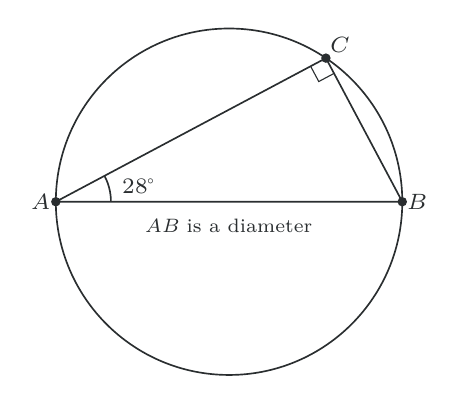
\begin{tikzpicture}[line width=0.6pt,ink,every node/.style={font=\footnotesize}]
\draw (0.000mm,0.000mm) circle (22.000mm);
\draw (-22.000mm,0.000mm) -- (22.000mm,0.000mm) -- (12.302mm,18.239mm) -- cycle;
\draw[ink,line width=0.4pt] (10.360mm,17.206mm) -- (11.393mm,15.264mm) -- (13.335mm,16.296mm);
\draw (-15.000mm,0.000mm) arc[start angle=0,end angle=28.000,radius=7mm];
\node[right] at (-14.800mm,1.900mm) {$28^\circ$};
\fill[ink] (-22.000mm,0.000mm) circle (0.6mm); \node[left,inner sep=1.5pt] at (-22.000mm,0.000mm) {$A$};
\fill[ink] (22.000mm,0.000mm) circle (0.6mm); \node[right,inner sep=1.5pt] at (22.000mm,0.000mm) {$B$};
\fill[ink] (12.302mm,18.239mm) circle (0.6mm); \node[above right,inner sep=1.5pt] at (12.302mm,18.239mm) {$C$};
\node[below=1pt] at (0.000mm,-0.500mm) {\scriptsize $AB$ is a diameter};
\end{tikzpicture}}}{$152$}{$124$}{$62$}{$56$}}
\meas{S2.7}{\satq{7}{From a point $E$ outside a circle with center $O$, tangent segments $\overline{EA}$ and $\overline{EU}$ are drawn to the circle, touching it at $A$ and $U$, with $\angle AEU=50^\circ$. Point $C$ lies on the major arc $AU$. What is the measure, in degrees, of $\angle ACU$?}{$130^\circ$}{$115^\circ$}{$65^\circ$}{$50^\circ$}}
\meas{S2.8}{\satg{8}{A circle has center $O$ and radius $6$. From a point $E$ outside the circle, tangent segments $\overline{EA}$ and $\overline{EU}$ of length $8$ are drawn (see the figure). Segment $\overline{OE}$ crosses the circle at $P$. What is the length of $\overline{PE}$?\figbox{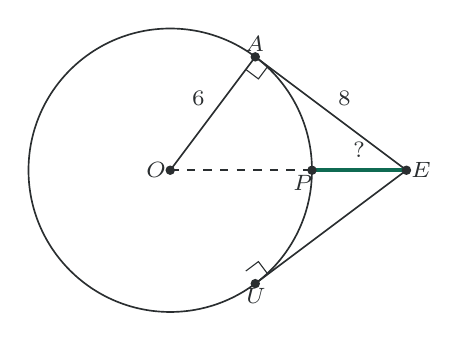
\begin{tikzpicture}[line width=0.6pt,ink,every node/.style={font=\footnotesize}]
\draw (0.000mm,0.000mm) circle (18.000mm);
\draw (0.000mm,0.000mm) -- (10.800mm,14.400mm) -- (30.000mm,0.000mm) -- (10.800mm,-14.400mm);
\draw[dashed] (0.000mm,0.000mm) -- (30.000mm,0.000mm);
\draw[accent,line width=1.4pt] (18.000mm,0.000mm) -- (30.000mm,0.000mm);
\draw[ink,line width=0.4pt] (9.600mm,12.800mm) -- (11.200mm,11.600mm) -- (12.400mm,13.200mm);
\draw[ink,line width=0.4pt] (9.600mm,-12.800mm) -- (11.200mm,-11.600mm) -- (12.400mm,-13.200mm);
\fill[ink] (0.000mm,0.000mm) circle (0.6mm); \node[left,inner sep=1.5pt] at (0.000mm,0.000mm) {$O$};
\fill[ink] (10.800mm,14.400mm) circle (0.6mm); \node[above,inner sep=1.5pt] at (10.800mm,14.400mm) {$A$};
\fill[ink] (10.800mm,-14.400mm) circle (0.6mm); \node[below,inner sep=1.5pt] at (10.800mm,-14.400mm) {$U$};
\fill[ink] (30.000mm,0.000mm) circle (0.6mm); \node[right,inner sep=1.5pt] at (30.000mm,0.000mm) {$E$};
\fill[ink] (18.000mm,0.000mm) circle (0.6mm); \node[below left,inner sep=1.5pt,xshift=1pt] at (18.000mm,0.000mm) {$P$};
\node[above left=-1pt] at (5.400mm,7.200mm) {$6$};
\node[above right=-1pt] at (20.400mm,7.200mm) {$8$};
\node[above=1pt] at (24.000mm,0.000mm) {$?$};
\end{tikzpicture}}}}
\meas{S2.9}{\satq{9}{A sector of a circle has a central angle of $60^\circ$ and an area of $24\pi$. What is the length of the arc of the sector?}{$4 \pi$}{$2 \pi$}{$12 \pi$}{$24 \pi$}}
\meas{S2.10}{\satq{10}{A sector of a circle has radius $9$ and a central angle of $\frac{5\pi}{6}$ radians. What is the area of the sector?}{$\frac{15 \pi}{4}$}{$\frac{15 \pi}{2}$}{$\frac{135 \pi}{2}$}{$\frac{135 \pi}{4}$}}
\meas{S2.11}{\satq{11}{A right triangle has legs of length $9$ and $12$. A circle is inscribed in the triangle, touching all three sides. What is the area of the part of the triangle that lies outside the circle?\figbox{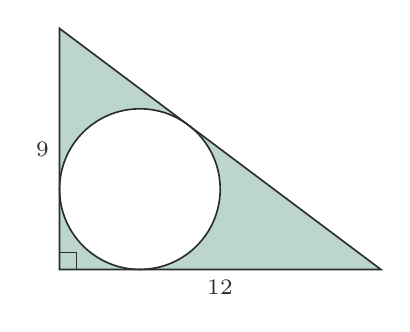
\begin{tikzpicture}[line width=0.6pt,ink,every node/.style={font=\footnotesize}]
\fill[accent!28] (0.000mm,0.000mm) -- (40.800mm,0.000mm) -- (0.000mm,30.600mm) -- cycle;
\filldraw[fill=white] (10.200mm,10.200mm) circle (10.200mm);
\draw (0.000mm,0.000mm) -- (40.800mm,0.000mm) -- (0.000mm,30.600mm) -- cycle;
\draw[ink,line width=0.4pt] (2.200mm,0.000mm) -- (2.200mm,2.200mm) -- (0.000mm,2.200mm);
\node[left] at (0.000mm,15.300mm) {$9$};
\node[below] at (20.400mm,0.000mm) {$12$};
\end{tikzpicture}}}{$54 - 36 \pi$}{$54 - 9 \pi$}{$54 - 6 \pi$}{$54 - 3 \pi$}}
\meas{S2.12}{\satq{12}{A circle in the $xy$-plane has center $(-4,6)$ and is tangent to the line $y=-2$. An equation of the circle is $(x+4)^2+(y-6)^2=k$. What is the value of $k$?}{$8$}{$16$}{$36$}{$64$}}
\meas{S2.13}{\satg{13}{Segment $\overline{PQ}$ with endpoints $P(1,2)$ and $Q(9,8)$ is a diameter of a circle in the $xy$-plane. The circle has equation $x^2+y^2+ax+by+c=0$, where $a$, $b$ and $c$ are constants. What is the value of $a+b+c$?}}
\meas{S2.14}{\satq{14}{In the $xy$-plane, the line $y=x+k$ is tangent to the circle $x^2+y^2=18$. Which of the following could be the value of $k$?}{$3 \sqrt{2}$}{$9$}{$18$}{$6$}}
\meas{S3.1}{\satq{1}{Two circles share the same center. A chord of the larger circle is tangent to the smaller circle and has length $24$ (see the figure). What is the area of the region between the two circles?\figbox{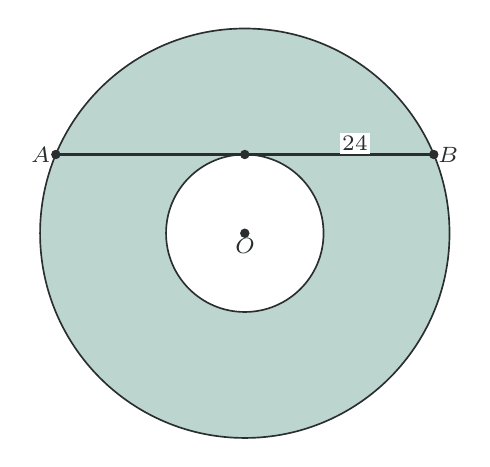
\begin{tikzpicture}[line width=0.6pt,ink,every node/.style={font=\footnotesize}]
\fill[accent!28,even odd rule] (0.000mm,0.000mm) circle (26.000mm) (0.000mm,0.000mm) circle (10.000mm);
\draw (0.000mm,0.000mm) circle (26.000mm); \draw (0.000mm,0.000mm) circle (10.000mm);
\draw[line width=0.9pt] (-24.000mm,10.000mm) -- (24.000mm,10.000mm);
\fill[ink] (0.000mm,0.000mm) circle (0.6mm); \node[below,inner sep=1.5pt] at (0.000mm,0.000mm) {$O$};
\fill[ink] (-24.000mm,10.000mm) circle (0.6mm); \node[left,inner sep=1.5pt] at (-24.000mm,10.000mm) {$A$};
\fill[ink] (24.000mm,10.000mm) circle (0.6mm); \node[right,inner sep=1.5pt] at (24.000mm,10.000mm) {$B$};
\fill[ink] (0.000mm,10.000mm) circle (0.6mm);
\node[above,fill=white,inner sep=1pt] at (14.000mm,10.000mm) {$24$};
\end{tikzpicture}}}{$12 \pi$}{$288 \pi$}{$576 \pi$}{$144 \pi$}}
\meas{S3.2}{\satq{2}{Four congruent circles lie inside a square of side $20$. Each circle touches the two nearest sides of the square and the two neighboring circles (see the figure). What is the area of the part of the square outside all four circles?\figbox{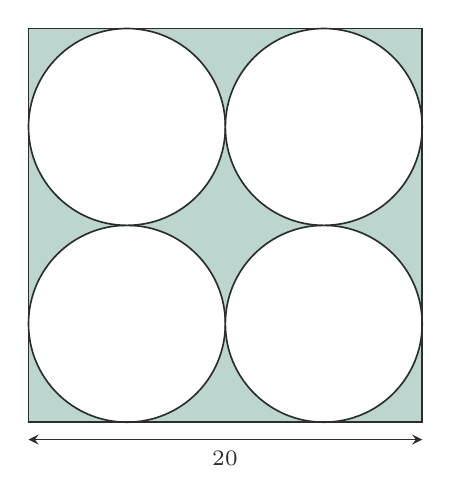
\begin{tikzpicture}[line width=0.6pt,ink,every node/.style={font=\footnotesize}]
\fill[accent!28] (0.000mm,0.000mm) rectangle (50.000mm,50.000mm);
\filldraw[fill=white] (12.500mm,12.500mm) circle (12.500mm);
\filldraw[fill=white] (12.500mm,37.500mm) circle (12.500mm);
\filldraw[fill=white] (37.500mm,12.500mm) circle (12.500mm);
\filldraw[fill=white] (37.500mm,37.500mm) circle (12.500mm);
\draw (0.000mm,0.000mm) rectangle (50.000mm,50.000mm);
\draw[<->,>=stealth] (0.000mm,-2.200mm) -- (50.000mm,-2.200mm) node[midway,below=0.5pt] {$20$};
\end{tikzpicture}}}{$400 - 25 \pi$}{$400 - 40 \pi$}{$400 - 100 \pi$}{$400 - 400 \pi$}}
\meas{S3.3}{\satq{3}{The figure shows a region made of a rectangle and two semicircles, one on each of the two short sides of the rectangle. The long side of the rectangle is $3$ times the short side. The perimeter of the whole region is $48+8\pi$. What is the area of the region?\figbox{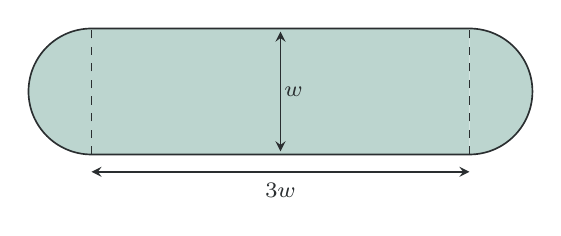
\begin{tikzpicture}[line width=0.6pt,ink,every node/.style={font=\footnotesize}]
\fill[accent!28] (0.000mm,0.000mm) rectangle (48.000mm,16.000mm);
\fill[accent!28] (48.000mm,0.000mm) arc[start angle=-90,end angle=90,radius=8.000mm] -- cycle;
\fill[accent!28] (0.000mm,0.000mm) arc[start angle=270,end angle=90,radius=8.000mm] -- cycle;
\draw (0.000mm,0.000mm) -- (48.000mm,0.000mm) arc[start angle=-90,end angle=90,radius=8.000mm] -- (0.000mm,16.000mm) arc[start angle=90,end angle=270,radius=8.000mm] -- cycle;
\draw[dashed] (0.000mm,0.000mm) -- (0.000mm,16.000mm); \draw[dashed] (48.000mm,0.000mm) -- (48.000mm,16.000mm);
\draw[<->,>=stealth] (24.000mm,0.400mm) -- (24.000mm,15.600mm) node[midway,right,inner sep=1pt] {$w$};
\draw[<->,>=stealth] (0.000mm,-2.200mm) -- (48.000mm,-2.200mm) node[midway,below=0.5pt] {$3w$};
\end{tikzpicture}}}{$192 + 8 \pi$}{$192 + 16 \pi$}{$192 + 32 \pi$}{$192 + 64 \pi$}}
\meas{S3.4}{\satg{4}{Square $ABCD$ has side length $12$. One arc of radius $12$ is centered at $A$ and passes through $B$ and $D$. A second arc of radius $12$ is centered at $C$ and also passes through $B$ and $D$ (see the figure). The area of the shaded region where the two arcs overlap is $a\pi-b$. What is the value of $a+b$?\figbox{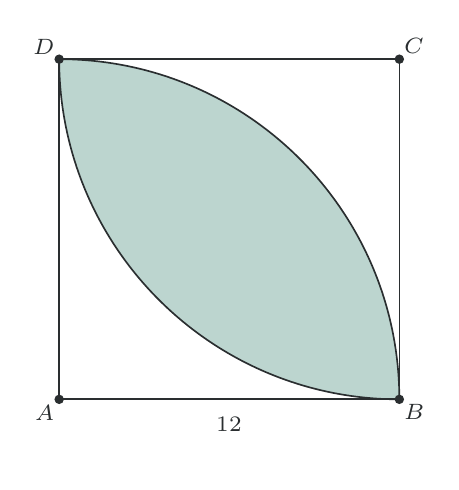
\begin{tikzpicture}[line width=0.6pt,ink,every node/.style={font=\footnotesize}]
\path[use as bounding box] (-4.000mm,-8.000mm) rectangle (47.200mm,47.200mm);
\begin{scope}\clip (0.000mm,0.000mm) circle (43.200mm); \fill[accent!28] (43.200mm,43.200mm) circle (43.200mm);\end{scope}
\draw (0.000mm,0.000mm) rectangle (43.200mm,43.200mm);
\draw (43.200mm,0.000mm) arc[start angle=0,end angle=90,radius=43.200mm];
\draw (0.000mm,43.200mm) arc[start angle=180,end angle=270,radius=43.200mm];
\fill[ink] (0.000mm,0.000mm) circle (0.6mm); \node[below left,inner sep=1.5pt] at (0.000mm,0.000mm) {$A$};
\fill[ink] (43.200mm,0.000mm) circle (0.6mm); \node[below right,inner sep=1.5pt] at (43.200mm,0.000mm) {$B$};
\fill[ink] (43.200mm,43.200mm) circle (0.6mm); \node[above right,inner sep=1.5pt] at (43.200mm,43.200mm) {$C$};
\fill[ink] (0.000mm,43.200mm) circle (0.6mm); \node[above left,inner sep=1.5pt] at (0.000mm,43.200mm) {$D$};
\node[below=1pt] at (21.600mm,-0.600mm) {$12$};
\end{tikzpicture}}}}
\meas{S3.5}{\satq{5}{A square with side length $10$ is inscribed in a circle (all four vertices lie on the circle). What is the area of the region inside the circle but outside the square?}{$50 \pi - 100$}{$50 \pi$}{$100 \pi - 100$}{$200 \pi - 100$}}
\meas{S3.6}{\satq{6}{Two circles have the same center. The radius of the larger circle is $25\%$ greater than the radius of the smaller circle. The region between the circles is what percent of the area of the larger circle?}{$25\%$}{$56.25\%$}{$64\%$}{$36\%$}}
\meas{S3.7}{\satq{7}{In the figure, $O$ is the center of a circle of radius $6$ and $\angle AOB=60^\circ$. What is the area of the shaded region bounded by chord $\overline{AB}$ and the minor arc $AB$?\figbox{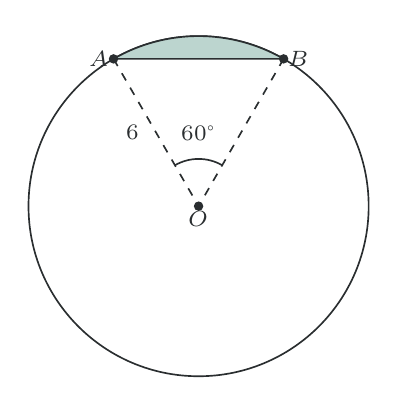
\begin{tikzpicture}[line width=0.6pt,ink,every node/.style={font=\footnotesize}]
\draw (0.000mm,0.000mm) circle (21.600mm);
\fill[accent!28] (10.800mm,18.706mm) arc[start angle=60.000,end angle=120.000,radius=21.600mm] -- cycle;
\draw (10.800mm,18.706mm) arc[start angle=60.000,end angle=120.000,radius=21.600mm] -- cycle;
\draw[dashed] (-10.800mm,18.706mm) -- (0.000mm,0.000mm) -- (10.800mm,18.706mm);
\draw (3.000mm,5.196mm) arc[start angle=60.000,end angle=120.000,radius=6mm];
\node at (0.000mm,9.200mm) {$60^\circ$};
\fill[ink] (0.000mm,0.000mm) circle (0.6mm); \node[below,inner sep=1.5pt] at (0.000mm,0.000mm) {$O$};
\fill[ink] (-10.800mm,18.706mm) circle (0.6mm); \node[left,inner sep=1.5pt] at (-10.800mm,18.706mm) {$A$};
\fill[ink] (10.800mm,18.706mm) circle (0.6mm); \node[right,inner sep=1.5pt] at (10.800mm,18.706mm) {$B$};
\node[left=1pt] at (-5.900mm,9.353mm) {$6$};
\end{tikzpicture}}}{$6 \pi$}{$6 \pi - 9$}{$6 \pi - 9 \sqrt{3}$}{$6 \pi - 18 \sqrt{3}$}}
\meas{S3.8}{\satg{8}{The radius of a circle is increased by $p\%$, and as a result the area of the circle increases by $69\%$. What is the value of $p$?}}
\meas{S3.9}{\satq{9}{An equilateral triangle with side length $6$ is inscribed in a circle (all three vertices lie on the circle). What is the area of the circle?}{$36 \pi$}{$12 \pi$}{$9 \pi$}{$3 \pi$}}
\meas{S3.10}{\satq{10}{Two circles with radii $4$ and $9$ are externally tangent. A line is tangent to the smaller circle at $P$ and to the larger circle at $Q$, and both circles lie on the same side of the line (see the figure). What is the length of $\overline{PQ}$?\figbox{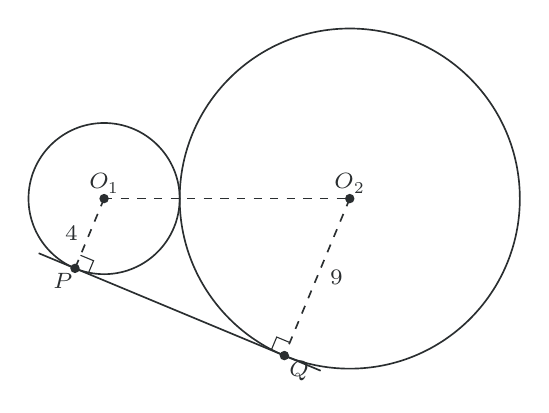
\begin{tikzpicture}[line width=0.6pt,ink,every node/.style={font=\footnotesize}]
\draw (0.000mm,0.000mm) circle (9.600mm); \draw (31.200mm,0.000mm) circle (21.600mm);
\draw (-8.308mm,-6.938mm) -- (27.508mm,-21.862mm);
\draw[dashed] (0.000mm,0.000mm) -- (-3.692mm,-8.862mm); \draw[dashed] (31.200mm,0.000mm) -- (22.892mm,-19.938mm);
\draw[dashed] (0.000mm,0.000mm) -- (31.200mm,0.000mm);
\draw[ink,line width=0.4pt] (-3.000mm,-7.200mm) -- (-1.338mm,-7.892mm) -- (-2.031mm,-9.554mm);
\draw[ink,line width=0.4pt] (23.585mm,-18.277mm) -- (21.923mm,-17.585mm) -- (21.231mm,-19.246mm);
\fill[ink] (0.000mm,0.000mm) circle (0.6mm); \node[above,inner sep=1.5pt] at (0.000mm,0.000mm) {$O_1$};
\fill[ink] (31.200mm,0.000mm) circle (0.6mm); \node[above,inner sep=1.5pt] at (31.200mm,0.000mm) {$O_2$};
\fill[ink] (-3.692mm,-8.862mm) circle (0.6mm); \node[below left,inner sep=1.5pt] at (-3.692mm,-8.862mm) {$P$};
\fill[ink] (22.892mm,-19.938mm) circle (0.6mm); \node[below right,inner sep=1.5pt] at (22.892mm,-19.938mm) {$Q$};
\node[left=0.5pt] at (-1.846mm,-4.431mm) {$4$};
\node[right=0.5pt] at (27.346mm,-9.969mm) {$9$};
\end{tikzpicture}}}{$5$}{$6$}{$12$}{$13$}}
\meas{S3.11}{\satg{11}{The radii of two circles are in the ratio $2:3$. The sum of the areas of the two circles is $52\pi$. What is the radius of the smaller circle?}}
\meas{S3.12}{\satq{12}{A rectangle with sides $16$ and $12$ is inscribed in a circle (all four vertices lie on the circle). What is the area of the region inside the circle but outside the rectangle?}{$64 \pi - 192$}{$100 \pi - 192$}{$100 \pi - 96$}{$400 \pi - 192$}}
\meas{S3.13}{\satg{13}{A circular rug has a diameter of $240$ centimeters. Its area is $k\pi$ square meters. What is the value of $k$?}}
\meas{S3.14}{\satq{14}{Circle $A$ is inscribed in a square (it touches all four sides). Circle $B$ is circumscribed about the same square (it passes through all four vertices). The area of circle $B$ is how many times the area of circle $A$?}{$\sqrt{2}$}{$2 \sqrt{2}$}{$4$}{$2$}}
\meas{S4.1}{\satq{1}{A right circular cylinder with radius $5$ and height $12$ has the same volume as a second right circular cylinder with height $3$. What is the radius of the second cylinder?}{$10$}{$20$}{$25$}{$100$}}
\meas{S4.2}{\satq{2}{A right circular cone has slant height $13$ and a base with diameter $10$. What is the volume of the cone?}{$100 \pi$}{$\frac{325 \pi}{3}$}{$300 \pi$}{$\frac{1300 \pi}{3}$}}
\meas{S4.3}{\satg{3}{A cylindrical tank has a base radius of $4$ decimeters and contains some water. A solid metal sphere of radius $3$ decimeters is lowered into the tank and sinks completely below the surface (no water spills). By how many decimeters does the water level rise? (Enter the exact decimal.)}}
\meas{S4.4}{\satq{4}{A solid metal cylinder with radius $6$ and height $8$ is melted and recast into solid spheres, each with radius $2$, with no metal lost. How many spheres are made?}{$54$}{$36$}{$27$}{$9$}}
\meas{S4.5}{\satq{5}{A scale model of a building is built at a scale of $1:50$, so every length on the model is $\frac1{50}$ of the matching length on the real building. The floor area of the model is $0.6$ square meters. What is the floor area, in square meters, of the real building?}{$75{,}000$}{$1{,}500$}{$30$}{$0.012$}}
\meas{S4.6}{\satq{6}{A square pyramid has a base with side length $10$ and a height of $12$, with its apex directly above the center of the base. What is the total surface area of the pyramid (the four triangular faces plus the base)?}{$260$}{$340$}{$360$}{$620$}}
\meas{S4.7}{\satg{7}{A container is an inverted right circular cone (point down) with height $12$ (see the figure). It is filled with water to a depth of $6$. The water fills what percent of the container's volume? (Enter the number without the percent sign.)\figbox{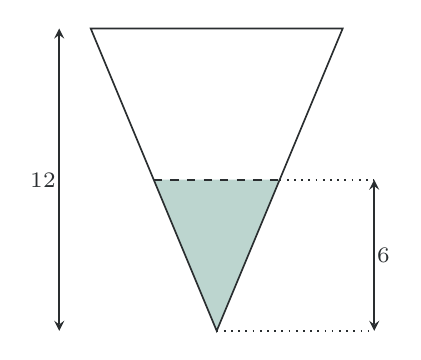
\begin{tikzpicture}[line width=0.6pt,ink,every node/.style={font=\footnotesize}]
\fill[accent!28] (0.000mm,0.000mm) -- (-8.000mm,19.200mm) -- (8.000mm,19.200mm) -- cycle;
\draw (0.000mm,0.000mm) -- (-16.000mm,38.400mm) -- (16.000mm,38.400mm) -- cycle;
\draw[dashed] (-8.000mm,19.200mm) -- (8.000mm,19.200mm);
\draw[<->,>=stealth] (-20.000mm,0.000mm) -- (-20.000mm,38.400mm) node[midway,left,inner sep=1pt] {$12$};
\draw[<->,>=stealth] (20.000mm,0.000mm) -- (20.000mm,19.200mm) node[midway,right,inner sep=1pt] {$6$};
\draw[dotted] (8.000mm,19.200mm) -- (20.000mm,19.200mm);
\draw[dotted] (0.000mm,0.000mm) -- (20.000mm,0.000mm);
\end{tikzpicture}}}}
\meas{S4.8}{\satq{8}{A rectangular tank has a base that measures $2$ meters by $1.5$ meters. Water flows into the tank at a constant rate of $45$ liters per minute. How many minutes does it take for the water level to rise $0.3$ meter? ($1$ cubic meter $=1000$ liters)}{$200$}{$20$}{$2$}{$0.02$}}
\meas{S4.9}{\satq{9}{The surface area of a sphere is increased by $125\%$. By what percent does the volume of the sphere increase?}{$125\%$}{$337.5\%$}{$406.25\%$}{$237.5\%$}}
\meas{S4.10}{\satg{10}{A closed right circular cylinder has a height of $10$ and a total surface area of $192\pi$ (both circular bases and the curved side). What is the radius of the cylinder?}}
\meas{S4.11}{\satg{11}{A circular sector with radius $10$ and central angle $288^\circ$ is cut out of paper, and its two straight edges are joined to form a right circular cone. The volume of the cone is $k\pi$. What is the value of $k$?}}
\meas{S4.12}{\satq{12}{A sphere fits snugly inside a right circular cylinder: it touches the top, the bottom and the curved side of the cylinder (see the figure). The volume of the cylinder is $432\pi$. What is the volume of the sphere?\figbox{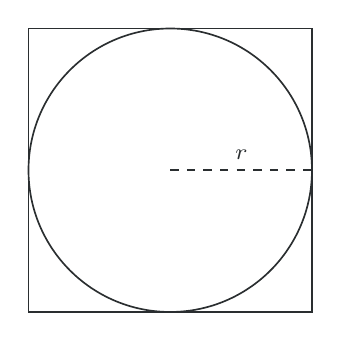
\begin{tikzpicture}[line width=0.6pt,ink,every node/.style={font=\footnotesize}]
\draw (-18.000mm,0.000mm) rectangle (18.000mm,36.000mm);
\draw (0.000mm,18.000mm) circle (18.000mm);
\draw[dashed] (0.000mm,18.000mm) -- (18.000mm,18.000mm);
\node[above=0pt] at (9.000mm,18.000mm) {$r$};
\end{tikzpicture}}}{$144 \pi$}{$216 \pi$}{$288 \pi$}{$576 \pi$}}
\meas{S4.13}{\satq{13}{A rectangular tank has a base $40$ cm by $25$ cm and contains water to a depth of $8$ cm. A solid cube with edge length $10$ cm is placed flat on the bottom of the tank. To the nearest tenth of a centimeter, what is the new depth of the water, measured from the bottom of the tank?}{$8.9$}{$8.0$}{$9.0$}{$10.0$}}
\meas{S4.14}{\satq{14}{A cylindrical can has a diameter of $8$ centimeters and a height of $15$ centimeters. To the nearest hundredth of a liter, how much does the can hold when full? ($1$ liter $=1000$ cubic centimeters)}{$0.19$}{$0.75$}{$3.01$}{$7.54$}}
\meas{S5.1}{\satg{1}{Two parallel chords of a circle have lengths $24$ and $10$. The chords lie on opposite sides of the center of the circle, and the distance between the chords is $17$ (see the figure). What is the radius of the circle?\figbox{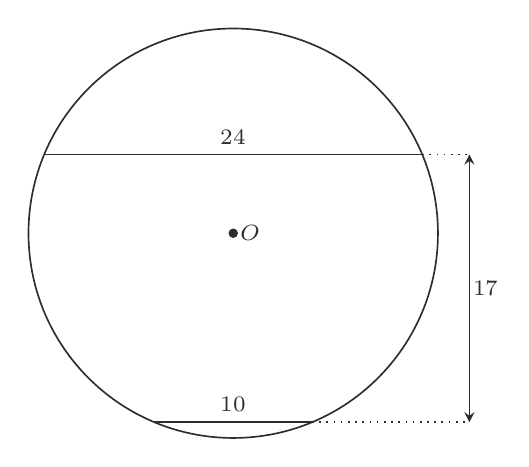
\begin{tikzpicture}[line width=0.6pt,ink,every node/.style={font=\footnotesize}]
\draw (0.000mm,0.000mm) circle (26.000mm);
\draw (-24.000mm,10.000mm) -- (24.000mm,10.000mm); \draw (-10.000mm,-24.000mm) -- (10.000mm,-24.000mm);
\fill[ink] (0.000mm,0.000mm) circle (0.6mm); \node[right,inner sep=1.5pt,xshift=1pt] at (0.000mm,0.000mm) {$O$};
\draw[dotted] (24.000mm,10.000mm) -- (30.000mm,10.000mm); \draw[dotted] (10.000mm,-24.000mm) -- (30.000mm,-24.000mm);
\draw[<->,>=stealth] (30.000mm,-24.000mm) -- (30.000mm,10.000mm) node[midway,right,inner sep=1pt] {$17$};
\node[above] at (0.000mm,10.000mm) {$24$};
\node[above] at (0.000mm,-24.000mm) {$10$};
\end{tikzpicture}}}}
\meas{S5.2}{\satq{2}{In the first quadrant of the $xy$-plane, two different circles are each tangent to both the $x$-axis and the $y$-axis, and each passes through the point $(2,1)$. What is the sum of the areas of the two circles?}{$26 \pi$}{$25 \pi$}{$6 \pi$}{$36 \pi$}}
\meas{S5.3}{\satg{3}{A sector of a circle has area $12$ and arc length $6$. What is the measure, in radians, of the central angle of the sector?}}
\meas{S5.4}{\satq{4}{Four points $A$, $B$, $C$, $D$ lie in this order on a circle so that the arcs $AB$, $BC$, $CD$ and $DA$ (the arcs between consecutive points that contain no other of the four points) are in the ratio $1:2:3:4$. Chords $\overline{AC}$ and $\overline{BD}$ intersect at point $P$ inside the circle (see the figure). What is the measure, in degrees, of $\angle APB$?\figbox{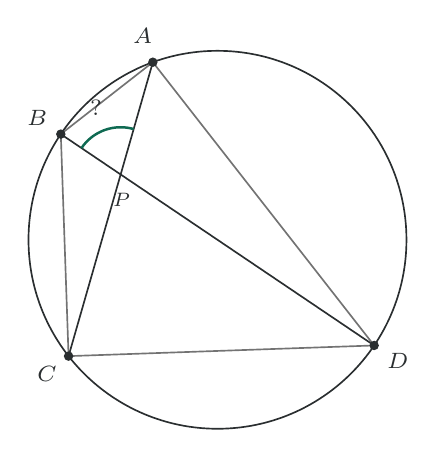
\begin{tikzpicture}[line width=0.6pt,ink,every node/.style={font=\footnotesize}]
\draw (0.000mm,0.000mm) circle (24.000mm);
\draw (-8.208mm,22.553mm) -- (-18.912mm,-14.776mm); \draw (-19.897mm,13.421mm) -- (19.897mm,-13.421mm);
\draw[black!55] (-8.208mm,22.553mm) -- (-19.897mm,13.421mm) -- (-18.912mm,-14.776mm) -- (19.897mm,-13.421mm) -- cycle;
\draw[accent,line width=0.9pt] (-10.643mm,14.062mm) arc[start angle=74.000,end angle=146.000,radius=6mm];
\node[inner sep=0pt] at (-15.375mm,16.752mm) {$?$};
\fill[ink] (-8.208mm,22.553mm) circle (0.6mm); \node[inner sep=0pt] at (-9.440mm,25.936mm) {$A$};
\fill[ink] (-19.897mm,13.421mm) circle (0.6mm); \node[inner sep=0pt] at (-22.881mm,15.434mm) {$B$};
\fill[ink] (-18.912mm,-14.776mm) circle (0.6mm); \node[inner sep=0pt] at (-21.749mm,-16.992mm) {$C$};
\fill[ink] (19.897mm,-13.421mm) circle (0.6mm); \node[inner sep=0pt] at (22.881mm,-15.434mm) {$D$};
\node[inner sep=0pt,xshift=0pt] at (-12.297mm,5.094mm) {\scriptsize $P$};
\end{tikzpicture}}}{$144^\circ$}{$108^\circ$}{$72^\circ$}{$36^\circ$}}
\meas{S5.5}{\satq{5}{A cylindrical tank has a radius of $3$ meters and a height of $4$ meters and is initially empty. An inlet pipe adds water at a constant rate of $6\pi$ cubic meters per hour while a drain removes water at a constant rate of $2\pi$ cubic meters per hour. Both run at the same time. How many hours does it take for the tank to be completely full?}{$4.5$}{$6$}{$18$}{$9$}}
\meas{S5.6}{\satq{6}{A solid sphere has a volume of $4500\pi$ cubic centimeters. A plane cuts the sphere at a distance of $9$ centimeters from the center of the sphere. What is the area, in square centimeters, of the circular cross-section made by the plane?}{$81 \pi$}{$144 \pi$}{$225 \pi$}{$306 \pi$}}
\meas{S5.7}{\satq{7}{A cube has edge length $6$. A sphere passes through all $8$ vertices of the cube. What is the volume of the sphere?}{$36 \pi$}{$108 \sqrt{3} \pi$}{$72 \sqrt{2} \pi$}{$288 \pi$}}
\meas{S5.8}{\satg{8}{Two similar solids have surface areas of $18$ and $50$. The volume of the smaller solid is $54$. What is the volume of the larger solid?}}
\meas{S5.9}{\satqw{9}{The radius of a right circular cylinder is increased by $10\%$ and its height is decreased by $20\%$. Which of the following describes the change in the volume of the cylinder?}{Decreases by $12\%$}{Decreases by $10\%$}{Decreases by $3.2\%$}{Does not change}}
\meas{S5.10}{\satq{10}{In the $xy$-plane, a circle has equation $x^2+y^2-4x-6y-12=0$. Point $P$ has coordinates $(15,3)$ and lies outside the circle. A line through $P$ touches the circle at exactly one point $T$. What is the length of $\overline{PT}$?}{$12$}{$5$}{$8$}{$13$}}
\meas{S5.11}{\satg{11}{A circle in the $xy$-plane passes through the points $(0,0)$, $(12,0)$ and $(0,5)$. What is the radius of the circle?}}
\meas{S5.12}{\satq{12}{A silo is a right circular cylinder with a hemisphere on top (see the figure). The base radius is $4$ feet, and the total height of the silo, from the ground to the top of the hemisphere, is $10$ feet. What is the volume of the silo, in cubic feet?\figbox{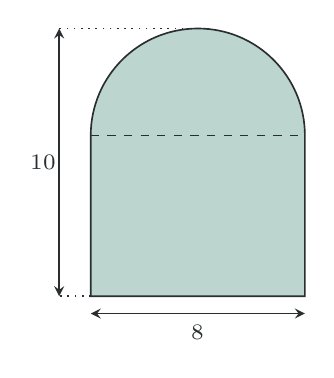
\begin{tikzpicture}[line width=0.6pt,ink,every node/.style={font=\footnotesize}]
\fill[accent!28] (-13.600mm,0.000mm) -- (13.600mm,0.000mm) -- (13.600mm,20.400mm) arc[start angle=0,end angle=180,radius=13.600mm] -- cycle;
\draw (-13.600mm,0.000mm) -- (13.600mm,0.000mm) -- (13.600mm,20.400mm) arc[start angle=0,end angle=180,radius=13.600mm] -- cycle;
\draw[dashed] (-13.600mm,20.400mm) -- (13.600mm,20.400mm);
\draw[<->,>=stealth] (-17.600mm,0.000mm) -- (-17.600mm,34.000mm) node[midway,left,inner sep=1pt] {$10$};
\draw[dotted] (-13.600mm,0.000mm) -- (-17.600mm,0.000mm); \draw[dotted] (0.000mm,34.000mm) -- (-17.600mm,34.000mm);
\draw[<->,>=stealth] (-13.600mm,-2.200mm) -- (13.600mm,-2.200mm) node[midway,below=0.5pt] {$8$};
\end{tikzpicture}}}{$224 \pi$}{$\frac{608 \pi}{3}$}{$\frac{544 \pi}{3}$}{$\frac{416 \pi}{3}$}}
\meas{S5.13}{\satq{13}{A cylindrical can with a radius of $10$ cm holds water to a depth of $9$ cm. All of the water is poured into an empty rectangular box whose base measures $15$ cm by $12$ cm. What is the depth, in cm, of the water in the box?}{$50 \pi$}{$20 \pi$}{$5 \pi$}{$5$}}
\meas{S5.14}{\satq{14}{A circle has radius $9$. The minor arc $AB$ has length $6\pi$. What is the length of chord $\overline{AB}$?}{$9 \sqrt{3}$}{$9$}{$9 \sqrt{2}$}{$18$}}
\meas{S5.15}{\satg{15}{A regular hexagon with side length $6$ is inscribed in a circle (all six vertices lie on the circle). The area of the region inside the circle but outside the hexagon is $a\pi-b\sqrt3$. What is the value of $a+b$?}}
\meas{S5.16}{\satq{16}{A pyramid has a square base with side length $12$ and a height of $9$; its apex is directly above the center of the base. A plane parallel to the base cuts the pyramid at a height of $3$ above the base (see the figure). What is the area of the cross-section?\figbox{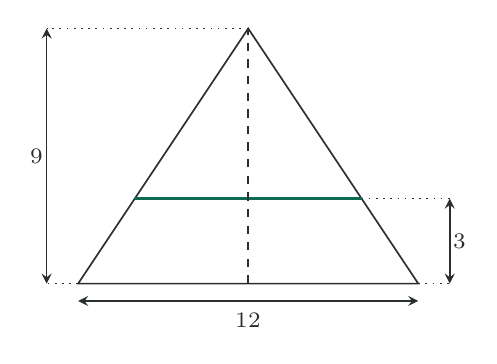
\begin{tikzpicture}[line width=0.6pt,ink,every node/.style={font=\footnotesize}]
\draw (-21.600mm,0.000mm) -- (21.600mm,0.000mm) -- (0.000mm,32.400mm) -- cycle;
\draw[accent,line width=1.2pt] (-14.400mm,10.800mm) -- (14.400mm,10.800mm);
\draw[dashed] (0.000mm,0.000mm) -- (0.000mm,32.400mm);
\draw[<->,>=stealth] (-21.600mm,-2.200mm) -- (21.600mm,-2.200mm) node[midway,below=0.5pt] {$12$};
\draw[<->,>=stealth] (-25.600mm,0.000mm) -- (-25.600mm,32.400mm) node[midway,left,inner sep=1pt] {$9$};
\draw[dotted] (-21.600mm,0.000mm) -- (-25.600mm,0.000mm); \draw[dotted] (0.000mm,32.400mm) -- (-25.600mm,32.400mm);
\draw[<->,>=stealth] (25.600mm,0.000mm) -- (25.600mm,10.800mm) node[midway,right,inner sep=1pt] {$3$};
\draw[dotted] (14.400mm,10.800mm) -- (25.600mm,10.800mm);
\draw[dotted] (21.600mm,0.000mm) -- (25.600mm,0.000mm);
\end{tikzpicture}}}{$8$}{$64$}{$16$}{$96$}}
\meas{S5.17}{\satg{17}{A right circular cone has height $12$. A plane parallel to the base cuts off a small cone at the top; the plane is $4$ units below the apex. The small cone has volume $8\pi$. The remaining solid (the frustum) has volume $k\pi$. What is the value of $k$?}}
\meas{S5.18}{\satq{18}{A container is an inverted right circular cone (point down) with top radius $6$ cm and height $9$ cm. It is initially empty and water flows in at a constant rate of $12\pi$ cubic centimeters per minute. How many minutes does it take for the water depth to reach $4.5$ cm?}{$13.5$}{$9$}{$4.5$}{$1.125$}}
\meas{S5.19}{\satq{19}{Two circles have the same center and radii $4$ and $10$. Two radii of the larger circle form an angle of $72^\circ$. What is the area of the part of the region between the two circles that lies inside this $72^\circ$ angle?}{$\frac{12 \pi}{5}$}{$\frac{36 \pi}{5}$}{$\frac{84 \pi}{5}$}{$84 \pi$}}
\meas{S5.20}{\satq{20}{A sector of a circle has an area of $36$ and a central angle of $2$ radians. What is the perimeter of the sector (the arc length plus the two straight edges)?}{$12$}{$18$}{$24$}{$36$}}
\meas{K}{\setkicker{Set 2}{Percent change: chains, reversals and wording traps.}}
\immediate\closeout\mw
\end{document}